
\section{BNC-Steckverbinder}
\label{section:steckverbinder_bnc}
\begin{frame}%STARTCONTENT
Einsatz: Für Funkgeräte mit kleiner Leistung bis hinauf zum \qty{70}{\centi\metre}-Band und in der Messtechnik


\begin{figure}
    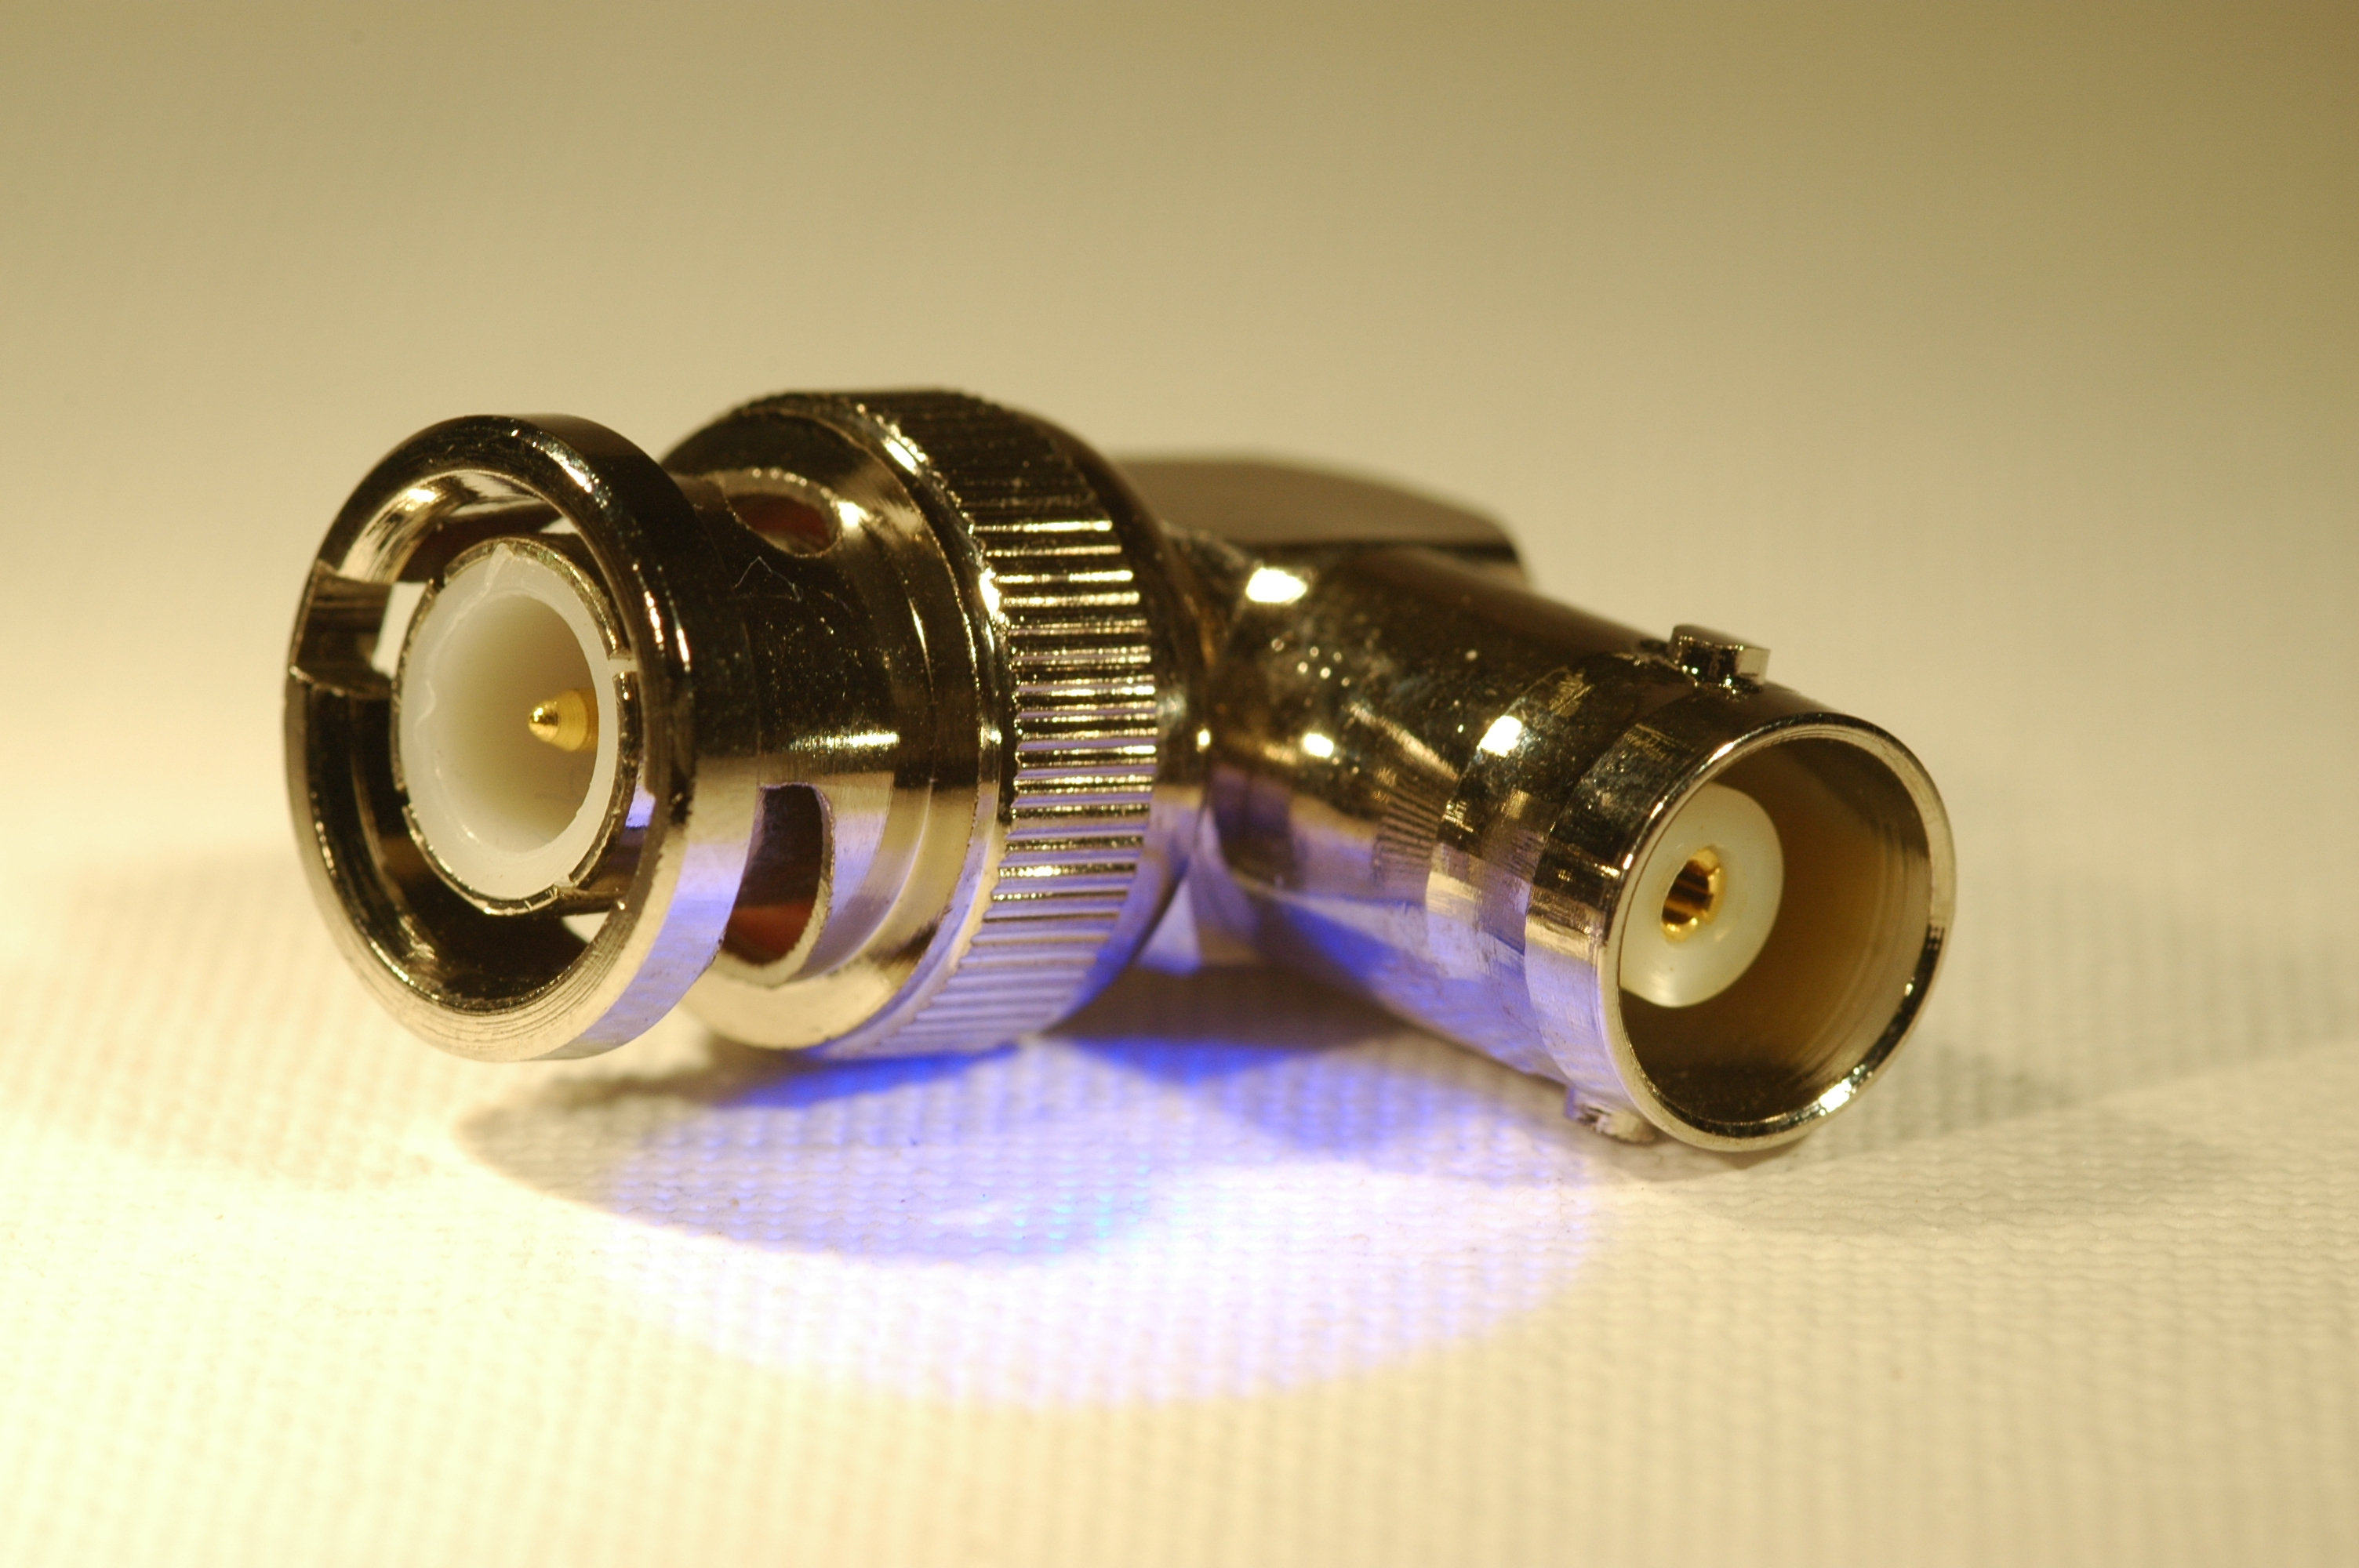
\includegraphics[width=0.85\textwidth]{foto/71}
    \caption{\scriptsize BNC-Winkeladapter mit Stecker links und Kupplung rechts}
    \label{n_koaxsteckverbinder_bnc}
\end{figure}

\end{frame}

\begin{frame}
\only<1>{
\begin{PQuestion}{NG203}{Welches HF-Steckverbindungs-System wird in der folgenden Darstellung gezeigt? }{N}
{SMA}
{PL}
{BNC}
{\DARCimage{1.0\linewidth}{608include}}\end{PQuestion}

}
\only<2>{
\begin{PQuestion}{NG203}{Welches HF-Steckverbindungs-System wird in der folgenden Darstellung gezeigt? }{N}
{SMA}
{PL}
{\textbf{\textcolor{DARCgreen}{BNC}}}
{\DARCimage{1.0\linewidth}{608include}}\end{PQuestion}

}
\end{frame}%ENDCONTENT
